% \usepackage{etex}
\usepackage{graphicx}
\usepackage[export]{adjustbox}
\usepackage{multicol}
% \usepackage{natbib}
% \usepackage[colorlinks]{hyperref}
% hyperref={colorlinks
\usepackage{bibentry}
\usepackage{subcaption}
% either subcaption or subfig only
% \usepackage{subfig}
% \usepackage{pdfpcnotes}
% \usepackage{pdfpages}
% \usepackage[dvipsnames]{xcolor}
\usepackage{pdfpcnotes}

\usepackage{xcolor}
\definecolor{ocre}{RGB}{110, 110, 110}
\usepackage{caption}
\usepackage[font={small,color=ocre},labelformat=empty]{caption}

\DeclareCaptionFont{black}{\color{black}}
\DeclareUnicodeCharacter{0301}{ì}

% \usepackage{minted}
% \usemintedstyle{pastie}

%% Titelbild
\titleimage{banner_pointnet3}

%% Gruppenlogo
\grouplogo{ISAS_logo}

% Beginn der Präsentation

\title[PointNet]{PointNet: Deep Learning on Point Sets for 3D Classification and Segmentation}
%\subtitle{entsprechend den Gestaltungsrichtlinien vom 1. August 2020}
\author[Felix Karg]{Felix Karg}
\supervisor{Antonio Zea}

\date[29.\,06.\,2022]{29. Juni 2022}

% Literatur

% citestyle
% - numbers: ieee, nature (science)
% \usepackage[citestyle=authoryear-comp,bibstyle=numeric,hyperref,backend=biber]{biblatex}
\usepackage[citestyle=alphabetic,bibstyle=numeric,hyperref,backend=biber]{biblatex}

\bibliography{references}
\addbibresource{references.bib}
% \addbibresource{../report/references.bib}
\bibhang1em


% Commands :)

\newcommand\blfootnote[1]{%
  \begingroup
  \renewcommand\thefootnote{}\footnote{\color{ocre}#1}%
  \addtocounter{footnote}{-1}%
  \endgroup
}

\newcommand\todo[1]{{\color{red}\textbf{TODO: #1}}}


\begin{document}

\begin{frame}[plain]
    \Large
    \textbf{The Need for 3D Deep Learning}
    \vspace{2em}
    \large
    \begin{figure}
    \captionsetup[subfigure]{labelformat=empty}
    \begin{subfigure}{0.3\textwidth}
        % lidar car visualization
        Robot Perception \\
        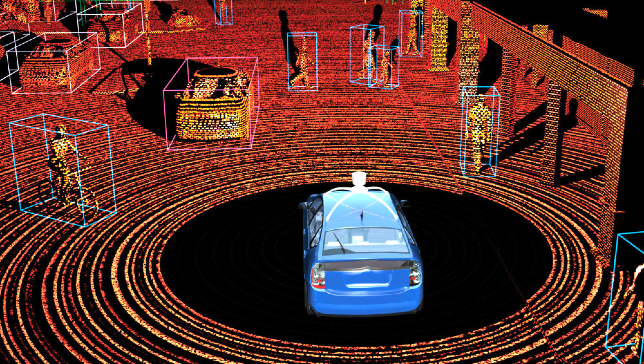
\includegraphics[height=0.35\textheight]{p02_6}
        \caption{source: Scott J Grunewald}
    \end{subfigure}
    \hspace{5mm}
    \begin{subfigure}{0.3\textwidth}
        % phone AR
        Augmented Reality \\
        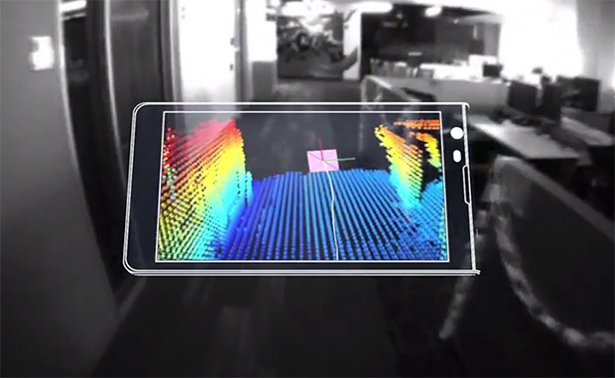
\includegraphics[height=0.35\textheight]{p02_8}
        \caption{source: Google Tango}
    \end{subfigure}
    \hspace{2mm}
    \begin{subfigure}{0.3\textwidth}
        % solidworks 3D objects
        Shape Design \\
        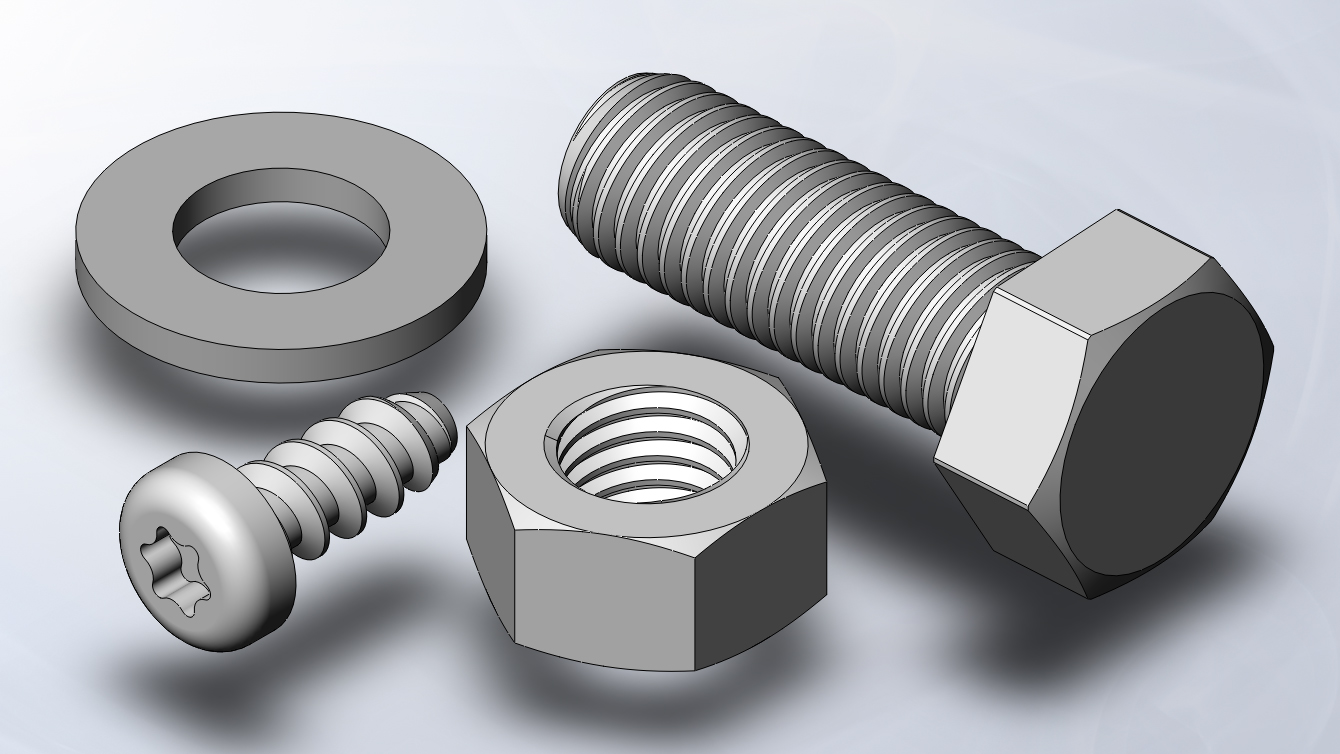
\includegraphics[height=0.35\textheight]{p02_7}
        \caption{source: solidworks}
    \end{subfigure}
    \blfootnote{Figures and captions from CVPR presentation to \cite{qi2017pointnet}.}
\end{figure}

    \Large
    \vspace{1em}
    A number of emerging 3D applications shape the need for 3D deep learning.
    \pnote{
        Es entstehen viele Anwendungen die Wahrnehmung  \\
        oder Interaktion in 3D benötigen, und damit bedarf \\
        für deep learning spezialisiert für räumliche Anwendungen \\
        shafft.
        \par
        - viele Anwendungen im 3D bereich entstehen \\
        - brauchen Wahrnehmung oder Interaktion in 3D \\
        - um diese zu bedienen: hoher bedarf \\
        - spezifisch auf 3D zugeschnitten \\
        - Erster: PointNet \\
    }
\end{frame}


% re-enable for more final versions
% Titelseite
\KITtitleframe
% \addtocounter{framenumber}{1}

%Inhaltsverzeichnis
% \begin{frame}{Inhaltsverzeichnis}
%     % \begin{multicols}{2}
%     \tableofcontents
%     % \end{multicols}
% \end{frame}

% \begin{frame}[c]{Agenda}
%     \hfill
%     \parbox[t]{.95\textwidth}{
%         \begin{minipage}[c][0.65\textheight]{\textwidth}
%             \tableofcontents
%         \end{minipage}
%         }
% \end{frame}
